\section{Learning on Graph-Structured Data}
\label{sec:graphresults}
% Added 20 Sep 2026.  Data, figure and table from
% code/implementation_3_algorithms/graph_learning.py and make_figures.py.
% No public benchmark (MUTAG, PTC) could be downloaded from the simulation
% environment -- the TU Dortmund, GitHub and HuggingFace mirrors are all
% blocked by its egress policy -- so the tasks are synthetic.  Rerun on a
% benchmark before any external claim is made.

The two application sections above exercise the walk on tabular and pixel
data, where the graph the walker moves on is chosen by the designer and the
data enter through the coin. The frame of the problem statement is
graph-structured data, where the graph \emph{is} the datum, and this section
tests the walk in that setting. The construction is the one the walk-based
kernels of Rossi et al.~\cite{Rossi_2013} and Bai et al.~\cite{Bai_2015}
use, transposed to discrete time: a walk is run on each graph and
permutation-invariant statistics of its evolution are the graph's
representation. A fidelity kernel $|\braket{\psi_G|\psi_{G'}}|^2$ between walk
states, of the kind used in Section~\ref{sec:kernelresults}, is not available
here --- it is undefined between graphs of different size and is not
invariant under vertex relabelling on graphs of the same size --- so the
statistics are what make the walk usable at all. The classical random walk is
given exactly the same statistics, which is the control that decides whether
the quantum walk contributes anything.

\paragraph*{Data and protocol.}
No public benchmark could be retrieved in the simulation environment, so the
data are three synthetic binary tasks on graphs of eight to twelve vertices,
one hundred graphs per class, with edge counts matched between classes so
that size and density alone do not separate them: random $3$-regular graphs
against Erd\H{o}s--R\'enyi graphs of the same edge count (\emph{regular});
random bipartite graphs against Erd\H{o}s--R\'enyi graphs of the same edge
count (\emph{bipartite}); and two-block stochastic block models with
$p_{\mathrm{in}} = 0.7$, $p_{\mathrm{out}} = 0.1$ against Erd\H{o}s--R\'enyi
graphs of the same expected density (\emph{community}). The coined walk uses
the Grover coin and the flip-flop shift of Section~\ref{sec:dtqw-graphs},
starts in the uniform superposition over arcs, and runs for $T = 8$ steps;
at each step the position marginal $p_t$ yields its Shannon entropy, its
inverse participation ratio and its maximum (each scaled by $n$), and $n$
further walks started at each vertex yield the mean return probability. The
$32$-dimensional signature is standardised and fed to an RBF support vector
machine; the classical control replaces the quantum walk by the lazy random
walk and the return probability by $\operatorname{tr}(P^t)/n$. Two further
baselines are the Weisfeiler--Lehman subtree kernel~\cite{Shervashidze_2011}
with three refinement rounds, and an RBF kernel on hand-made statistics (the
degree histogram, average clustering, spectral radius, smallest adjacency
eigenvalue and density). The walk network of the second experiment is the
same walk with one trainable coin angle per step, $C_t = \cos\theta_t\,
\mathbb{I} - i\sin\theta_t\,G$, followed by a logistic read-out of the
signature and trained end to end with COBYLA; its control fixes every
$\theta_t$ at the Grover value. All figures are the mean and standard
deviation of test accuracy over three repeats of stratified ten-fold
cross-validation, with the SVM grid chosen by an inner three-fold search.

\paragraph*{The walk signature is competitive, and the quantum walk edges
the classical one.}
Table~\ref{tab:graph} and Figure~\ref{fig:graphacc} give the result. The
regular task is trivial and every method is at or near $100$ per cent; it is
retained as a sanity check and carries no information. On the bipartite task
the discrete-time walk signature reaches $99.5 \pm 1.5$ per cent against the
classical walk's $97.7 \pm 3.3$, and on the community task $83.7 \pm 9.3$
against $82.7 \pm 7.3$. The quantum walk is ahead on both informative tasks,
but the margins are within one standard deviation over folds and the claim
is correspondingly weak: the quantum walk's statistics are at least as
informative as the classical walk's at equal step count, and slightly more
so on the two tasks that are not trivial. The WL kernel is the weakest
method on both, at $70.8$ and $64.8$ per cent, which is expected rather than
surprising --- these graphs carry no vertex labels, and the subtree kernel on
unlabelled graphs sees little beyond the degree sequence, which is matched by
construction on the bipartite task. The hand-made statistics match the
walks on bipartiteness, where the spectral symmetry $\lambda_{\min} =
-\lambda_{\max}$ decides the question exactly, and fall slightly behind on
the community task. The bipartite result deserves one mechanistic remark.
Before the return probability was added to the signature the walk kernels
scored in the low seventies on this task, well behind the spectral baseline;
the entropy, participation and maximum of the position distribution of a
walk started in the uniform arc state barely distinguish a bipartite graph
from a random one of the same density, and the return probability, which is
a spectral quantity, does. The signature is
therefore not a free lunch: which statistics are taken from the walk matters
as much as which walk is run.

\paragraph*{Training the coin adds nothing.}
The walk network with fixed Grover coins reaches $100$, $100$ and $84.0 \pm
7.8$ per cent on the three tasks; with the eight coin angles trained end to
end it reaches $100$, $100$ and $83.8 \pm 8.1$. The trainable coin is
therefore not the source of whatever the walk contributes, on these data, and
this is consistent with the finding of Section~\ref{sec:qnnresults} that
additional coin freedom enlarges the search space without enlarging the set
of reachable behaviours enough to pay for it. The optimiser was given sixty
evaluations per fold and started near the Grover point, so a better-trained
coin cannot be excluded; but a fairer statement is that on graphs of this
size the eight-step Grover walk already extracts what the read-out can use.

\paragraph*{What this does and does not show.}
The section establishes that a coined discrete-time walk, run with the same
tooling as the rest of the thesis, gives a graph representation that is at
least as good as its classical counterpart and better than the standard
unlabelled subtree kernel on structural tasks; it does not establish an
advantage on any benchmark that the literature uses, because none could be
obtained, and the synthetic tasks are small and easy enough that the
strongest classical baseline is within a few points on every one. The
kernels here are, as in the published quantum-walk kernels, classical
kernels on walk-derived invariants, and nothing in the construction requires
a quantum device: the walk is a $\dim = n d$ unitary on graphs of at most
twelve vertices and is simulated exactly. The result is a statement about
the walk as a feature extractor, not about quantum advantage.

\begin{figure}[htbp]
  \centering
  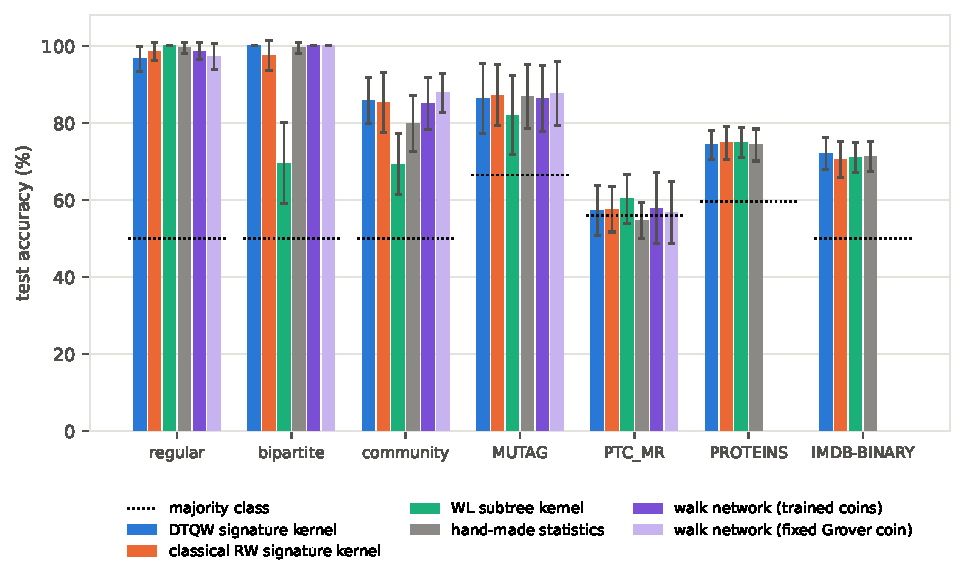
\includegraphics[width=\textwidth]{fig_graph_acc.pdf}
  \caption[Graph classification with walk signatures]{Test accuracy on the
  three synthetic graph-classification tasks, mean and standard deviation
  over thirty stratified folds. The dotted line is chance. Both walk
  signatures use $T = 8$ steps and the same four statistics per step.}
  \label{fig:graphacc}
\end{figure}

% Generated by make_figures.py -- do not edit by hand.
\begin{table}[htbp]
\centering\small
\caption{Graph classification on the three synthetic tasks: test accuracy (\%), mean $\pm$ s.d.\ over $3 \times 10$ stratified folds. Kernels are RBF--SVMs on the walk signature ($T=8$ steps, four statistics per step) or the WL subtree kernel ($h=3$); the walk network is the same walk with one trainable coin angle per step and a logistic read-out.}
\label{tab:graph}
\begin{tabular}{lrrr}
\hline
Method & regular & bipartite & community \\
\hline
DTQW signature kernel & $100.0 \pm 0.0$ & $99.5 \pm 1.5$ & $83.7 \pm 9.3$ \\
classical RW signature kernel & $99.5 \pm 1.5$ & $97.7 \pm 3.3$ & $82.7 \pm 7.3$ \\
WL subtree kernel & $100.0 \pm 0.0$ & $70.8 \pm 11.4$ & $64.8 \pm 8.0$ \\
hand-made statistics & $99.5 \pm 1.5$ & $99.7 \pm 1.2$ & $82.2 \pm 7.3$ \\
walk network (trained coins) & $100.0 \pm 0.0$ & $100.0 \pm 0.0$ & $83.8 \pm 8.1$ \\
walk network (fixed Grover coin) & $100.0 \pm 0.0$ & $100.0 \pm 0.0$ & $84.0 \pm 7.8$ \\
\hline
\end{tabular}
\end{table}


